\chapter{Example}
\label{example}
\pagenumbering{arabic}
\setcounter{page}{33}






\section{Stacking faults in LiNiO$_{2}$}

Lithium nickel oxide has been intensively studied as a positive electrode material in Li-ion batteries \cite{Whit2004}.
As other lithium transition metal oxides, it crystallizes in an O3-type layered structure consisting in three NiO$_{2}$ slabs per unit cell, with an ABCABC oxygen stacking sequence, and lithium ions located in the octahedral sites of the interlayer spaces (see figure \ref{estructura}). In order to explain the significant broadening of the (10\emph{l}) and (01\emph{l}) diffraction lines, DIFFaX simulations have been used for this material with the hypothesis of the existence of O1 stacking faults in the structure at low lithium concentrations (Li$_{\epsilon}$Ni$_{1.02}$O$_{2}$, $\epsilon\leq$ 0.3) \cite{Crog2000}. These stacking faults represent a break in the normal stacking sequence of the structure, with a local ABAB oxygen stacking sequence.

\begin{figure}[h!]
\begin{center}
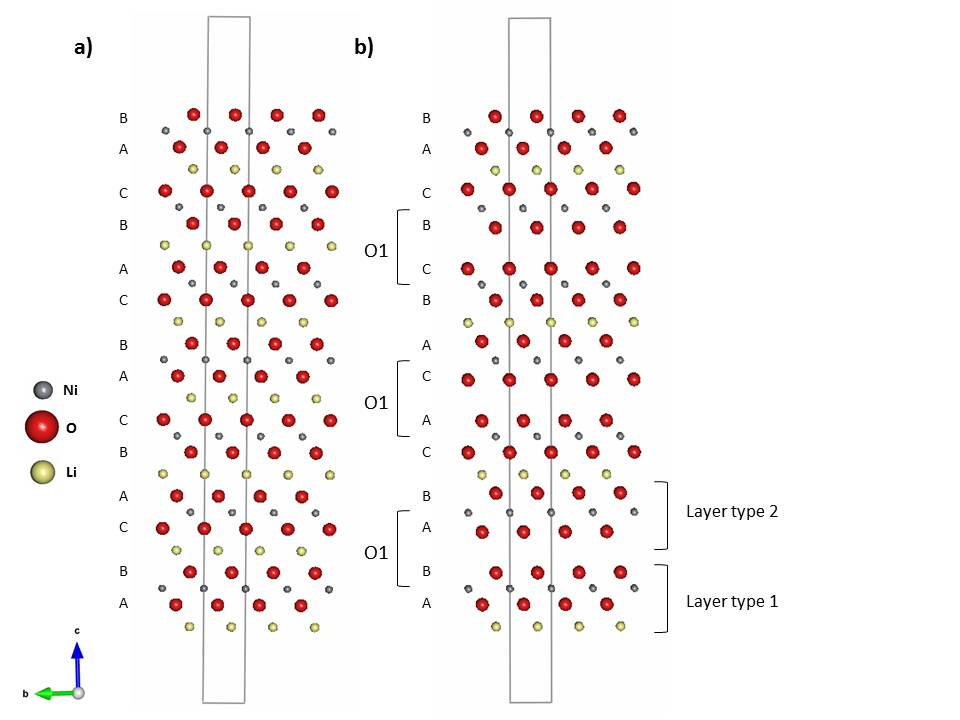
\includegraphics [width=5.3 in]{LiNO_estructura.jpg}
\caption{\bf a) Ideal structure of lithium nickel oxide (LiNiO$_{2}$) with O3 stacking, and b) defective structure with O1 stacking faults (Li$_{\epsilon}$Ni$_{1.02}$O$_{2}$).}
\label{estructura}
\end{center}
\end{figure}

The ideal structure can be described with three layers, each one containing a NiO$_{2}$ slab and a lithium interslab. The three layers are structurally identical, but shifted with respect to each other, resulting in transition vectors $\vec{t}_{12}$=$\vec{t}_{23}$=$\vec{t}_{31}$=(2/3 1/3 1/3) and a stacking probability of 1 for each transition. O1 defects require the definition of a new type of layer, structurally different, since these defective layers do not contain any lithium (see figure \ref{esquemacapes}). Therefore, three more layers are defined in the faulted structure, structurally identical between each other but different from the previous ones, and new transitions are allowed  in order to describe the defects (see figure \ref{capes}).

\begin{sidewaysfigure}
\begin{center}
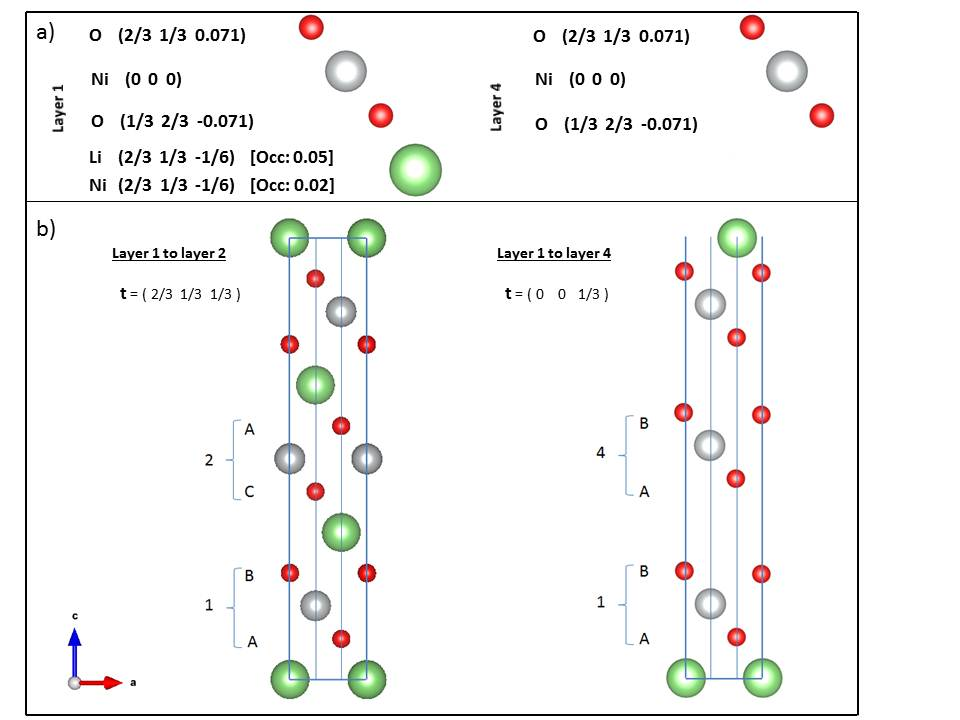
\includegraphics [width=6in]{description.jpg}
\caption{\bf  a) Schematic representation and atomic coordinates of the layers required for describing stacking faults for Li$_{0.05}$Ni$_{1.02}$O$_{2}$ in the FAULTS program. b) Graphic representation of the different transition possibilities from layer 1 and transition vectors.}
\label{esquemacapes}
\end{center}
\end{sidewaysfigure}

\begin{figure}[h!]
\begin{center}
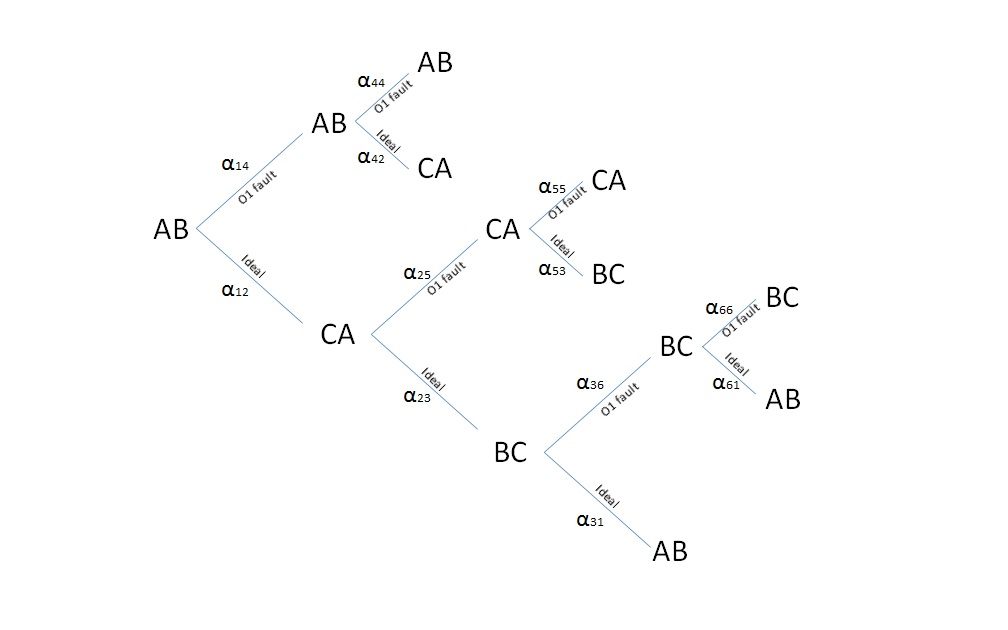
\includegraphics [width=5.2 in]{transitions.jpg}
\caption{\bf Possible layer transitions for Li$_{\epsilon}$Ni$_{1.02}$O$_{2}$ containing O1-type stacking faults, where $\alpha_{ij}$ is the probability transition from layer \emph{i} to layer \emph{j}.}
\label{capes}
\end{center}
\end{figure}





\section{Analysis of simulated data}
\label{Analysis of simulated data}

By  means of the  stacking description described above, FAULTS has been used to simulate a diffraction pattern with the parameter's values described in table \ref{taulasim}.
The obtained simulated XRD pattern for Li$_{\epsilon}$Ni$_{1.02}$O$_{2}$ ($\epsilon\leq$ 0.3) has then been used to analyse and test out the program. This are also the example files (LiNiO2$\_$simul.flts and LiNiO2$\_$refine.flts) included with the program. The refinement has been done by means of the Levenberg Marquart minimization algorithm, restraining the program to a maximum of 2400 function evaluations and a criterion of convergence 0.1e-4. As an example of the refinement process, the initial values of the refined parameters, which have been chosen far enough from the correct ones not to bias the result,
and  the final refined values are also  shown in table \ref{taulasim}.
A visual comparison between the calculated and the simulated powder patterns and their difference is shown in figure \ref{sim}.
Starting Rp and Chi$^{2}$ values were 45.62$\%$  and 186.38 respectively and reached a final value of 4.86$\%$ and 1.03 respectively.
The values of the refined parameters are very close to those used in the simulation and lead to a XRD pattern practically
identical to the one obtained with the values of these parameters used in the simulation (see figure \ref{sim}).



\begin{table}
\begin{center}
\begin{tabular}{|c|c|c|c|}
\hline
Refined parameter & Simulation & Initial value & Final value(Std dev.)\\

\hline
a,b & 2.81540 & 2.86540 & 2.81510(10)\\
\hline
c & 13.363000 & 13.26300 & 13.3638(7)\\
\hline
Scale & 1.00000 & 1.00000 & 1.010(3)\\
\hline
z$_{O1}$,z$_{O3}$ & 0.07133	&0.17133&	0.0716(2)\\
\hline
z$_{O2}$,z$_{O4}$ & -0.07133	&-0.17133& -0.0716(2)\\
\hline
$\alpha_{12}$,$\alpha_{23}$,$\alpha_{31}$ & 0.8580&	1.0000	&0.8569(10)\\
\hline
$\alpha_{14}$,$\alpha_{25}$,$\alpha_{36}$ & 0.1420&	0.0000	&0.1431(10)\\
\hline
$\alpha_{42}$,$\alpha_{53}$,$\alpha_{61}$ & 0.8580&	1.0000	&0.842(6)\\
\hline
$\alpha_{44}$,$\alpha_{55}$,$\alpha_{66}$ & 0.1420&	0.0000	&0.158(6)\\
\hline


\end{tabular}
\caption{\textbf{Starting and final values of the parameters refined in the analysis of simulated data.}}
\label{taulasim}
\end{center}
\end{table}


\begin{sidewaysfigure}
\begin{center}
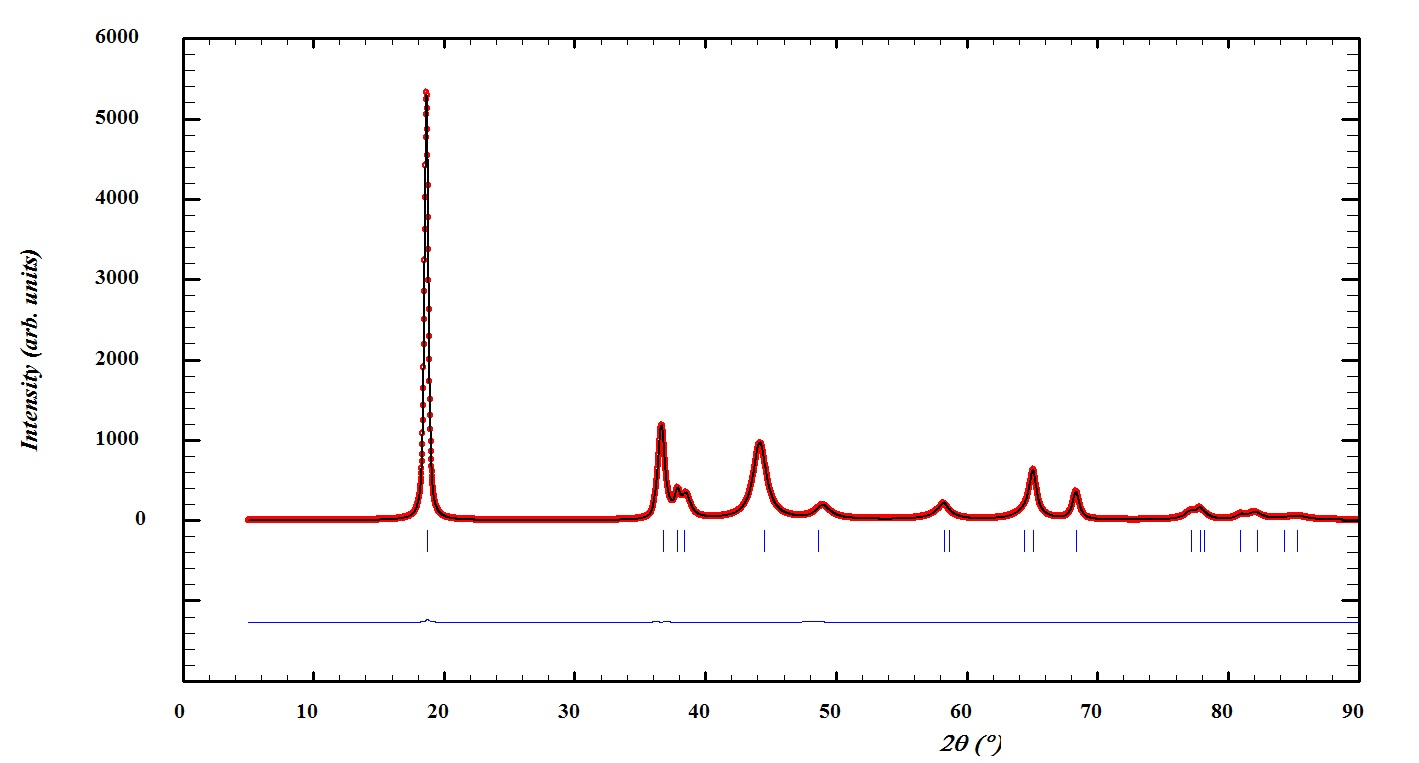
\includegraphics [width=6 in]{pattern.jpg}
\caption{\bf Comparison of the X-ray diffraction patterns corresponding to the FAULTS analysis of the simulated data: simulated pattern (dotted curve) and calculated pattern using the FAULTS refinement (continuous curve). The diagram underneath shows the difference between them. The ticks show the position of the Bragg reflections of the R-3m average unit cell (the one used to describe the ideal O3 structure of Li$_{\epsilon}$Ni$_{1.02}$O$_{2}$).  }
\label{sim}
\end{center}
\end{sidewaysfigure}

An example of the evolution of \textit{a} and \textit{b} cell parameters and of Chi$^{2}$ and Rp throughout a run of 12 iteration cycles is shown in \ref{cycles}.

\begin{figure}[!htbp]
\begin{center}
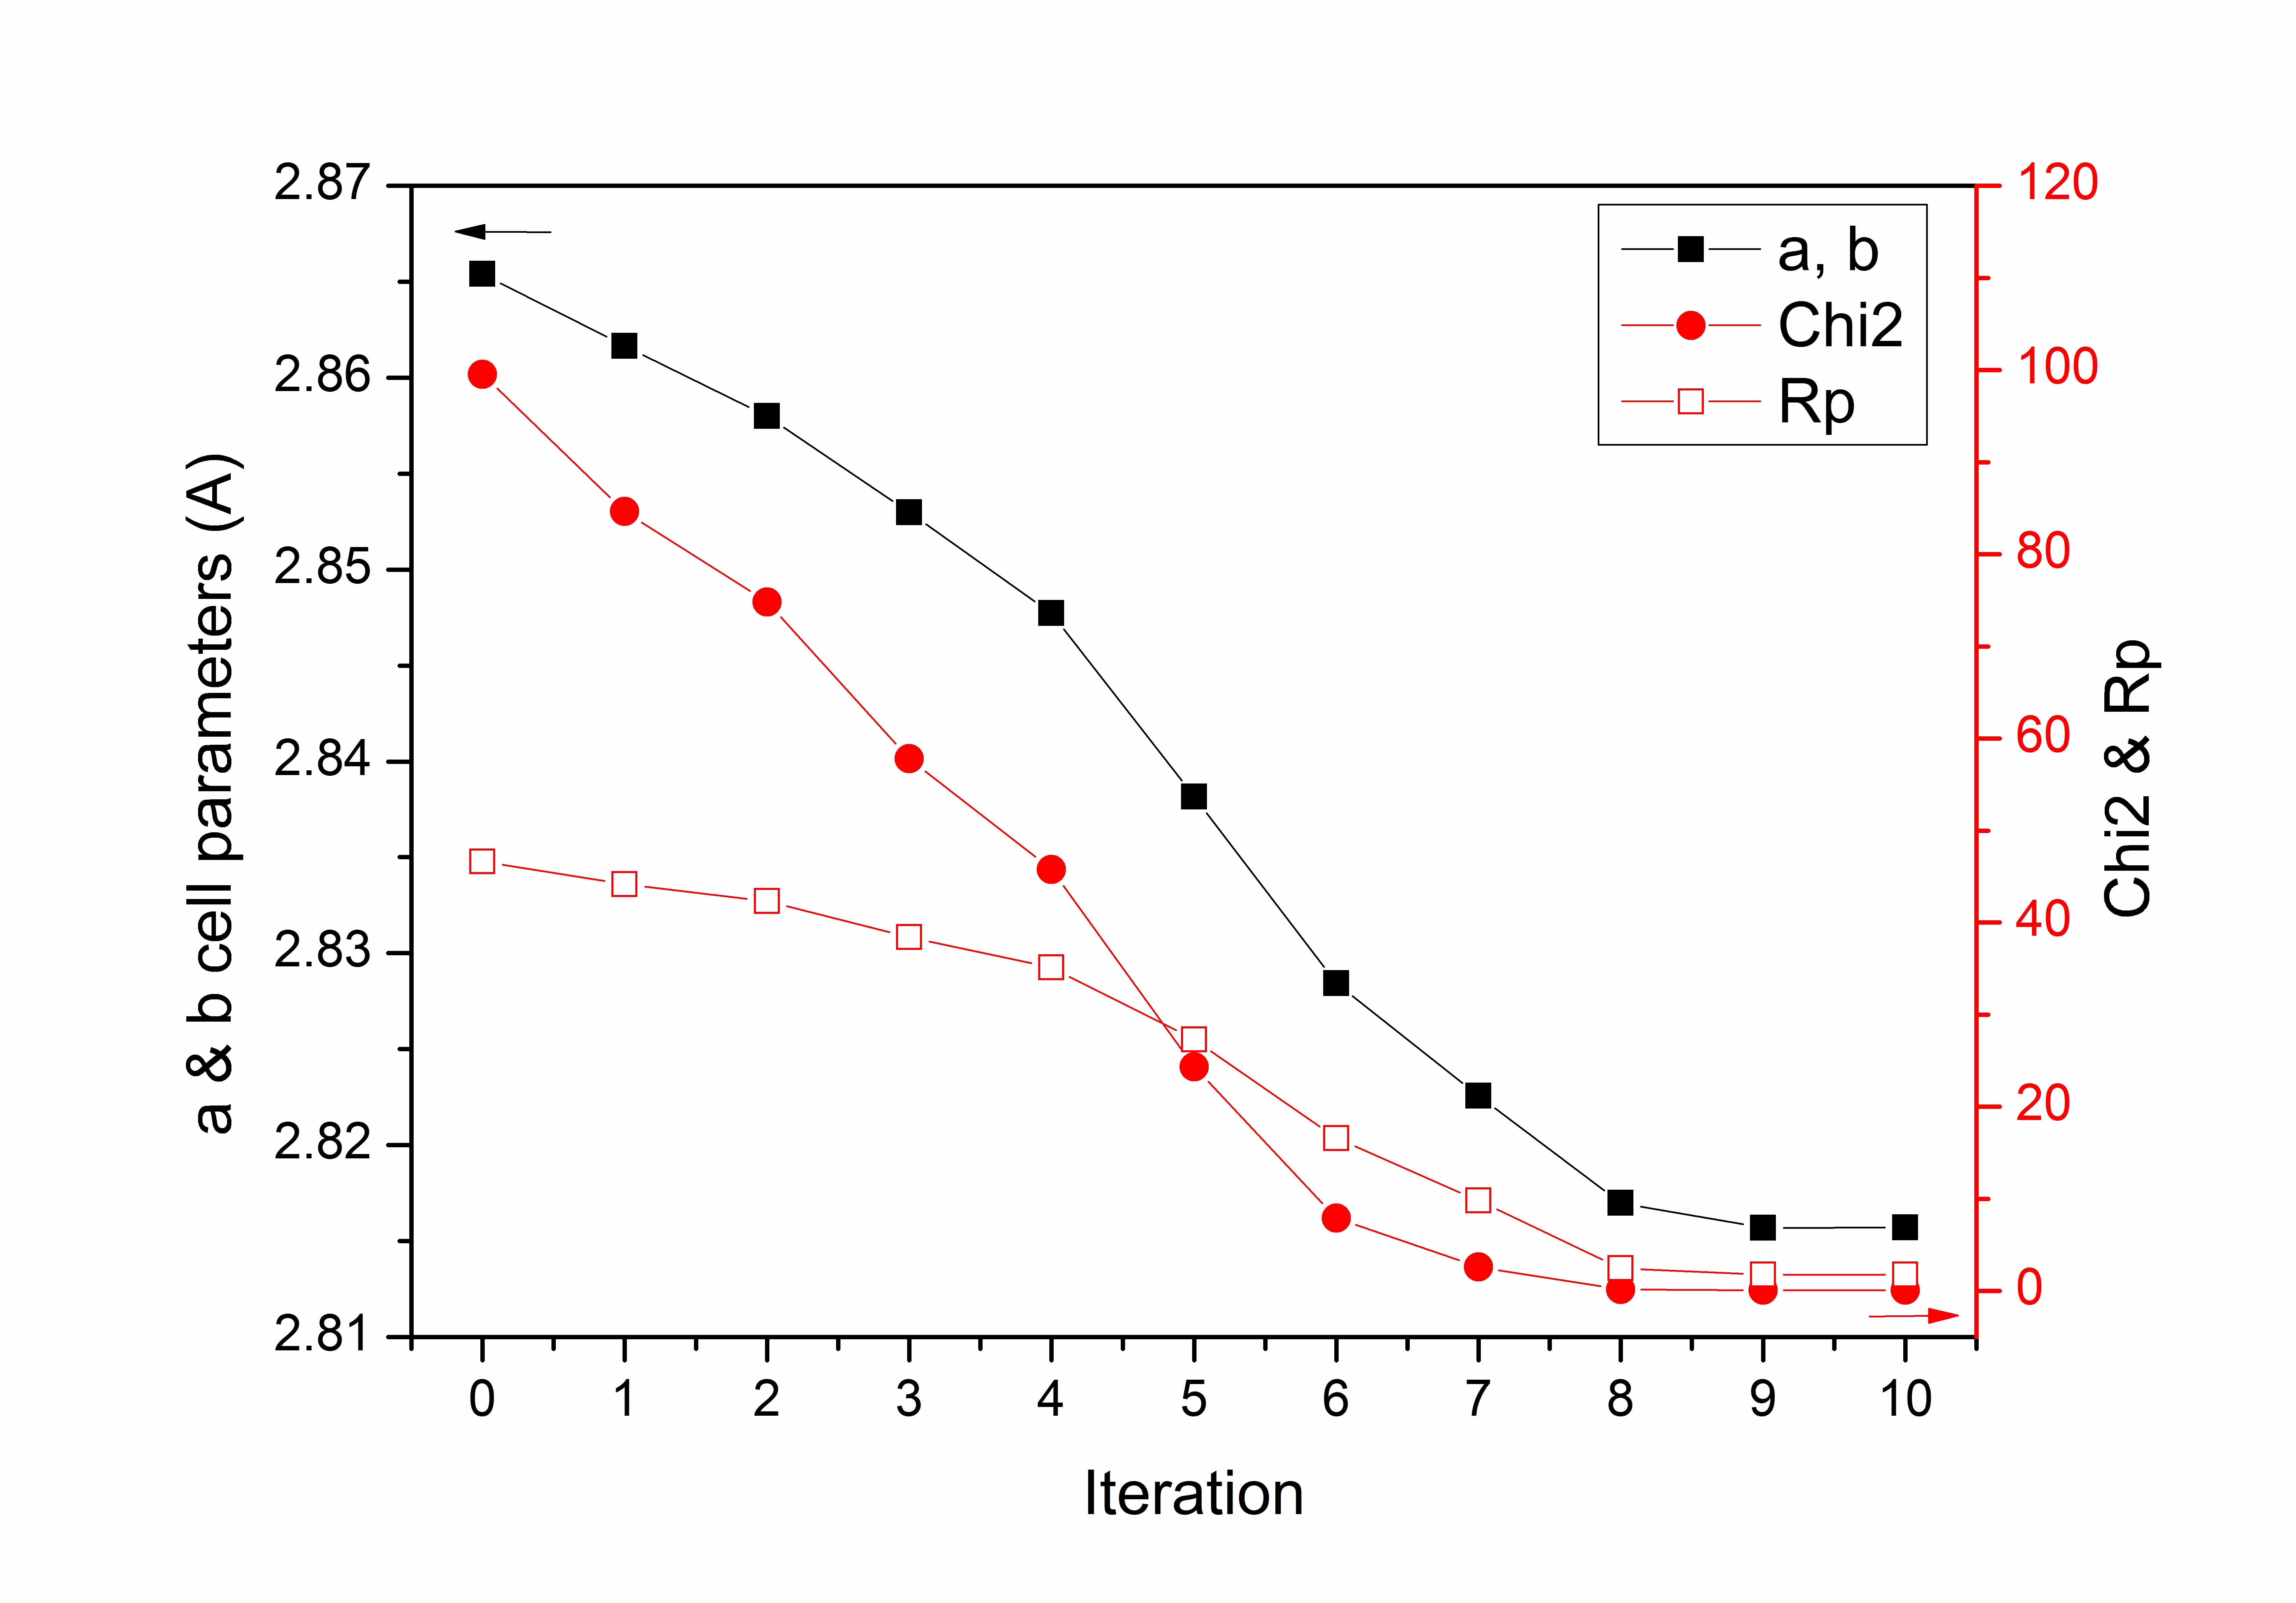
\includegraphics [width=4 in]{chi2_Rf.jpg}
\caption{\bf Evolution of the functions Rp and Chi$^{2}$ and of the cell parameters a and b, versus the cycle number. }
\label{cycles}
\end{center}
\end{figure}
